\section{Replay Buffer}
\label{appendix:replay_buffer}

Within each iteration, sampling a large number of trajectories from a single question can lead to imbalanced training, causing the model to overfit to specific samples. To address this issue, we introduce a replay buffer mechanism that distributes sampled trajectories across multiple iterations, ensuring a more balanced question distribution, as shown in Figure \ref{fig:replay_buffer}. Additionally, PPO's clip mechanism helps maintain stable optimization when using these trajectories from previous iterations. Specifically, in our experiments, we use a \emph{6-6-6} tree structure for sampling, generating $6 \times 6 \times 6 = 216$ trajectories per question. In each iteration, we sample 16 distinct questions to generate trajectories, and these trajectories are then distributed across the following 8 iterations, with at most 32 trajectories per question processed in each iteration. As a result, each iteration covers 128 distinct questions (8 × 16), ensuring a well-balanced sample distribution. We observe that the clip ratio remains around 0.1, validating the effectiveness of our replay buffer strategy.

Our replay buffer mechanism leads to a certain degree of off-policy learning, enabling our framework to be compatible with the asynchronous RL setting, which was first explored by \cite{noukhovitch2025asynchronousrlhffasterefficient}. Leveraging asynchronous RL can further parallelize data collection and policy optimization, potentially leading to additional efficiency improvements.

\begin{figure}[t]
  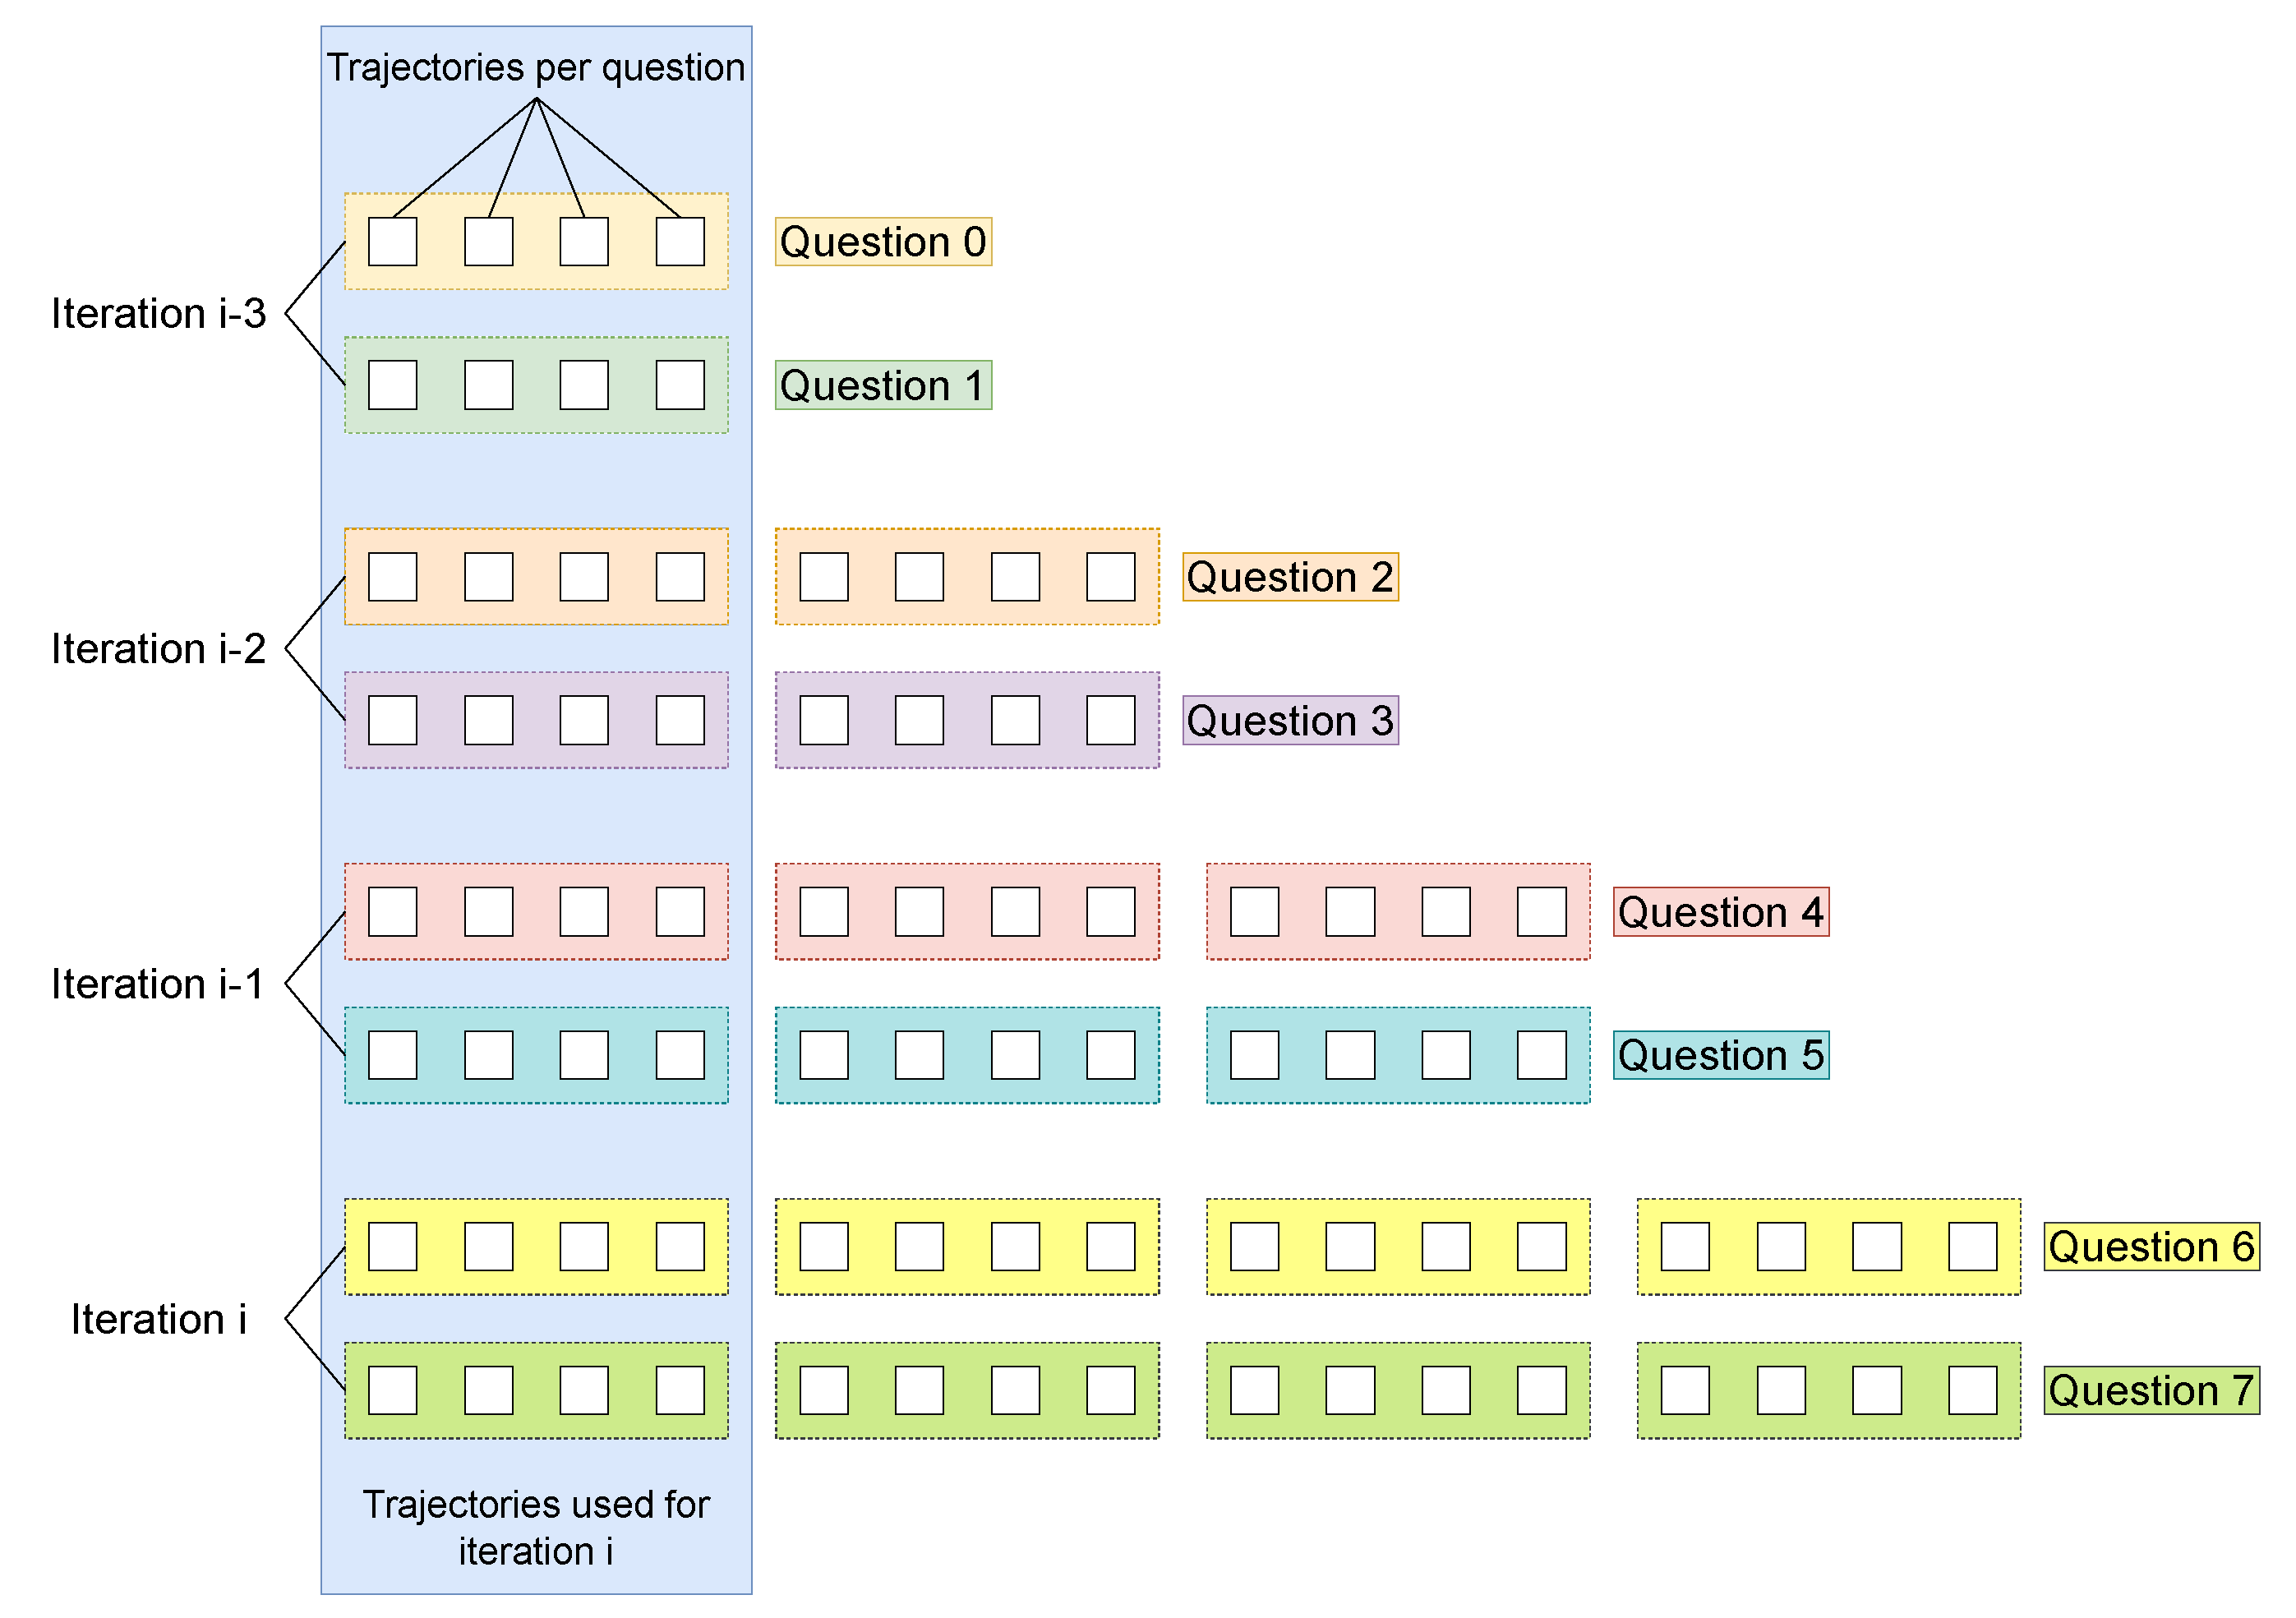
\includegraphics[width=\textwidth]{figures/replay_buffer.drawio.pdf}
  \caption{Illustration of the replay buffer. In this example, in each iteration, we sample two questions, with each question generating four trajectories. These trajectories are distributed across four iterations for optimization. The trajectories used in the $i$-th iteration are selected in the blue box. In total, there are 8 different questions, each with 4 trajectories, ensuring a balanced distribution of samples.}
  \label{fig:replay_buffer}
\end{figure}